\label{sec:introdutction}
In recent years, the capabilities of a single agent have been significantly improved. To further expand the capabilities of intelligent robots, using several robots can accelerate many tasks, such as localization, exploration, and mapping.
Decentralized visual simultaneous localization and
mapping (DSLAM) can share location and environmental information between robots and is the essential task for many multi-robot applications. \cite{Cieslewski:20187ee} concludes the basic procedure as \cref{fig:all}

\begin{figure}[h]  
    \centering  
    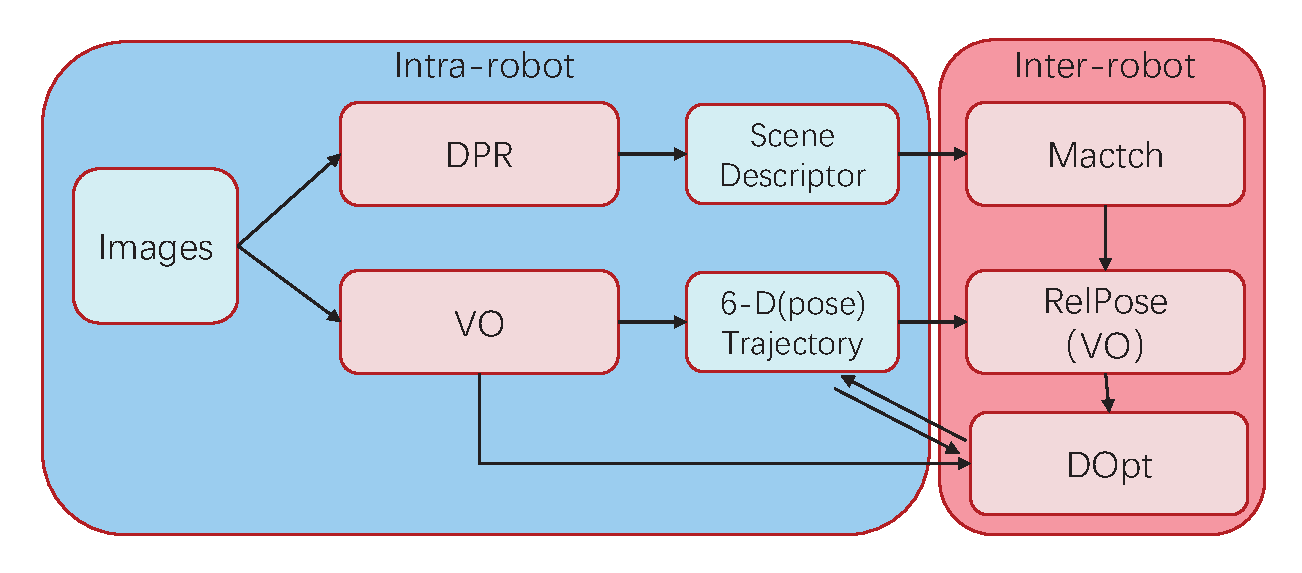
\includegraphics[width=0.75\linewidth]{fig/all.eps}
    \caption{DSLAM framework\cite{Cieslewski:20187ee}. \textbf{VO} is used to calculate the intra-robot 6-D absolute pose from the input frames. \textbf{DPR} produces a compact image representation that communicate among robots. \textbf{Match} stage finds out candidate inter-robot place recognition matches.  \textbf{RelPose} requires data from the matched robots and establishes relative poses between the robots trajectories. \textbf{DOpt} obtains the trajectories, intra-robot pose measurements from VO and inter-robot relative poses from RelPose, and updates the trajectories.}
    \label{fig:all}
\end{figure}

There are five components: DPR, VO, Match, RelPose and DOpt. DPR and VO are intra-robot operations, and require high computation resources on embedded system. Match, RelPose and DOpt are inter-robot operations, and consume most of the communication of DSLAM sytem. The RelPose components can and should depend the VO components since it can benefit from re-using the data and computation resources of VO.

The previous work \cite{Cieslewski:20187ee} uses ORB-SLAM\cite{Mur-Artal:2017281} as the VO and NetVLAD\cite{Arandjelovic:2017997} as the DPR component. These two algorithms both consume a large amount of computation and storage, and pose a great challenge to DSLAM on the embedded system. The DSLAM frame in \cite{Cieslewski:20187ee} is illustrated in \cref{fig:all_pre}.


\begin{figure*}[thb]
    \begin{minipage}[t]{0.5\linewidth}  
    \centering
    \subfigure[DSLAM in \cite{Cieslewski:20187ee}] {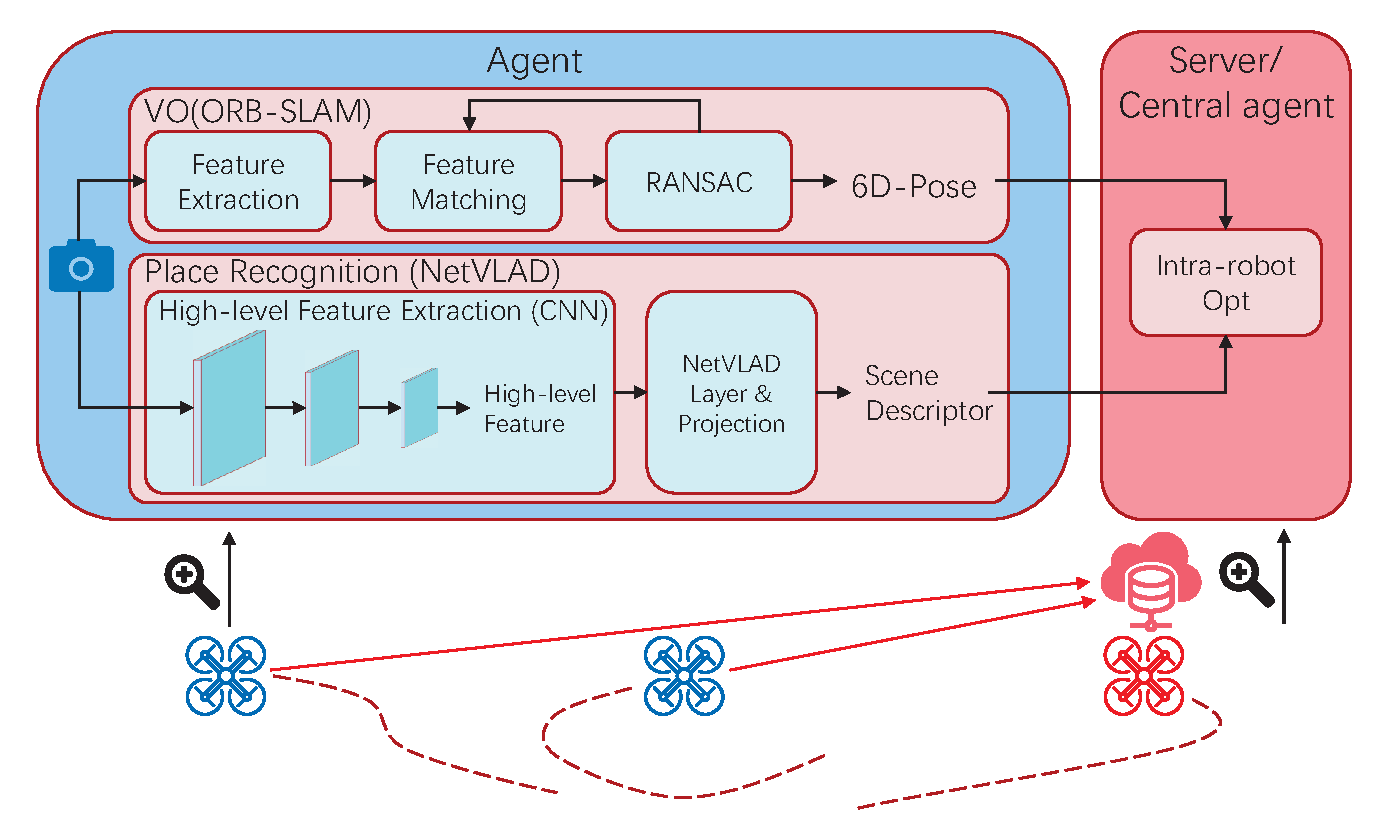
\includegraphics[width=1\textwidth]{fig/overview_pre.eps}\label{fig:all_pre}}
    \end{minipage}
    \begin{minipage}[t]{0.5\linewidth}  
    \centering  
    \subfigure[Our CNN-based DSLAM.] {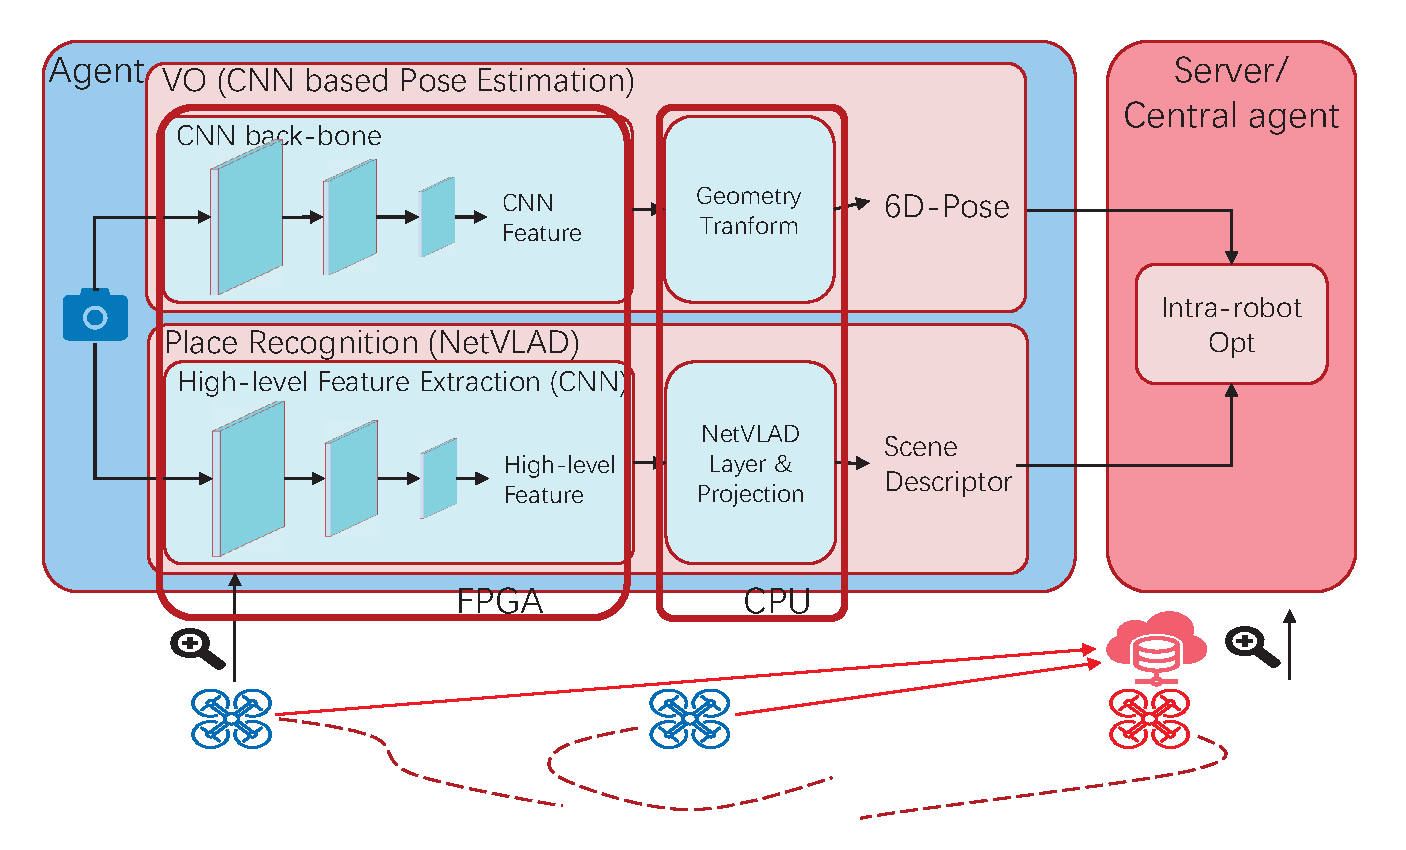
\includegraphics[width=1\linewidth]{fig/overview_us.eps}\label{fig:all_us}} 
    \end{minipage}
    \caption{(a) The previous work uses ORB feature-point based method to estimate the trajectory from the sequence of the stereo camera, and use NetVLAD \cite{Arandjelovic:2017997} to do DPR. (b) Our framework adopt Depth-VO-Feat \cite{Zhan:2018e92} in DSLAM system as the monocular VO, and we use the same method of NetVLAD in \cite{Cieslewski:20187ee} to do DPR. We use Xilinx Zynq MPSoC hardware platform to for deployment.
    }
\label{fig:overview}
\end{figure*}

Monocular systems are much easier to deploy than binocular systems. The transitional monocular feature point based VO should use complex depth reconstruction methods to compute the absolute scale of the pose scale\cite{pizzoli2014remode}, leading to speed-down. With the development of CNN, we can reconstruct the depth and pose with the absolute scale from the monocular camera directly, making monocular VO more robust and efficient\cite{Zhan:2018e92}. ecent advances in deep learning and the availability of large labelled visual datasets have significantly improved the accuracy of place recognition, such as NetVLAD\cite{Arandjelovic:2017997}. However, previous works concentrate on the accuracy of the CNNs, yet consider little about the deployment CNNs on the embedded system.

Though DSLAM system can benefit from the development of CNN, the fully CNN-based DSLAM system faces some key issues: 1) The embedded system usually support fixed-point CNN. 2) The speed will decline in the embedded system when running several CNN models simultaneously, the speed-down of DPR will lead to the decline of the final DSLAM accuracy. Therefore, we build up a CNN-based monocular DSLAM system on embedded FPGA platform, with following contributions:

\begin{itemize}
\item To the best of our knowledge, this work is the first to implement all components of monocular DSLAM with CNN.
% We adopt Depth-VO-Feat \cite{Zhan:2018e92} in DSLAM system to estimate the pose from the input monocular camera. We use the same method of NetVLAD in  \cite{Cieslewski:20187ee} to do place recognition. 
We deploy the system on Xilinx Zynq MPSoC hardware platform with DPU \cite{Tech:2019360}, which is an embedded CNN accelerator. The proposed DSLAM framework is illustrated in \cref{fig:all_us}.
\item As the embedded system usually support fixed-point CNN, we propose a pose-sensitive fixed-point fine-tune method to make the feature extraction layers fixed-point and remain the pose prediction layers floating-point, reaching the same accuracy with the original floating-point VO network. We schedule the fixed-point layers on DPU and the floating-point layers on CPU, so that we can accelerate the VO to 10ms.
\item To increase the NetVLAD frequency, we propose a cross-components scheduling method to scheduling the computation flow across VO and DPR, as well as across the PL and PS of MPSoC to make full use of the embedded platform. We calculate the NetVLAD every 4 input frames from every 6 frames, improving the final accuracy of DSLAM. 
We also propose a new indicator called loop-closure recall (LCR), which indicates the remaining rate of loop-closure after trajectory merging, to evaluate the performance of trajectory merging. The output result of DSLAM with different NetVLAD frequency is illustrated in \cref{fig:dslamresult}. The tranditional average trajectory error (ATE) can not indicate the performance of trajectory merging in DSLAM.
\end{itemize}



\begin{figure}[thb]
    \begin{minipage}[t]{0.475\linewidth}  
    \centering
    \subfigure[NetVLAD/8 frames. \protect\          ATE=9] {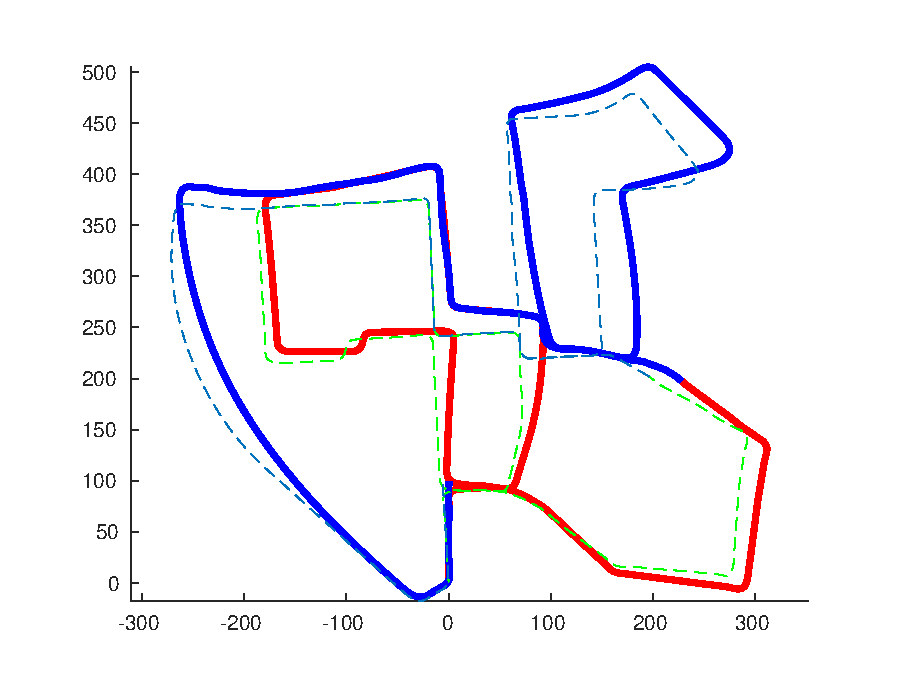
\includegraphics[width=1\linewidth]{fig/8netvlad.eps}\label{fig:8netvlad}}
    \end{minipage}
    \begin{minipage}[t]{0.475\linewidth}  
    \centering  
    \subfigure[NetVLAD/12 frames. \protect\ ATE=9] {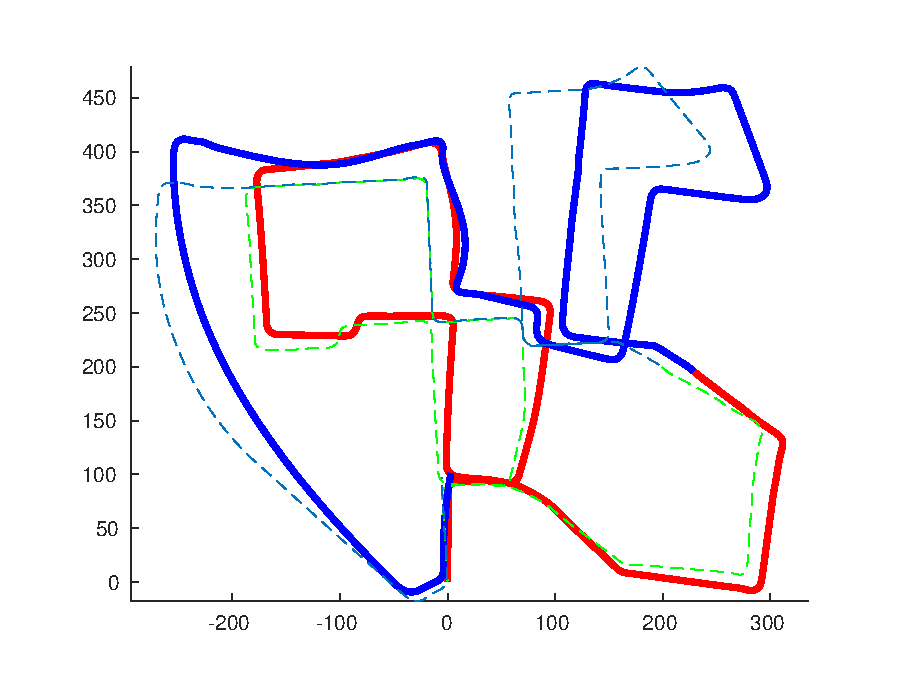
\includegraphics[width=1\linewidth]{fig/12netvlad.eps}\label{fig:12netvlad}} 
    \end{minipage}
    \caption{The DSLAM result of two robots(red and blue, the dashed is the ground truth the robots). (a) When do NetVLAD every 8 frames, the trajectories can be merged correctly. (b) When do NetVLAD every 12 frames, the trajectories can not be commendably merged. However, the ATE of these two results is similar.
    }
\label{fig:dslamresult}
\end{figure}



% The rest part of this article is orgnized as follows. \Cref{sec:background} will give the basic idea of CNN based methods and the hardware architecture of embedded platform, Xilinx Zynq MPSoC. \Cref{sec:hardsoft} will detail the implementation of our pose-sensitive fixed-point fine-tune method and the cross-components scheduling method. The experiment results will be given in \Cref{sec:experiment}. \Cref{sec:conclusion} will conclude this paper.